\chapter{Evaluation}
\label{chap:evaluation}

This chapter evaluates our hybrid retrieval system for validation rules using a preliminary test set of 30 queries. We assess retrieval quality through ranking metrics, optimize weights via Leave-One-Out Cross-Validation, and validate system performance characteristics.

\section{Evaluation Setup}
\label{sec:evaluation-setup}

\subsection{Dataset}

Our evaluation uses 30 test queries with manually annotated ground truth, where each query has exactly one correct target rule. While this dataset is small for definitive conclusions, it provides initial validation of our approach and methodology for future larger-scale evaluation.

\paragraph{Query characteristics:}
\begin{itemize}[leftmargin=*,itemsep=2pt,topsep=2pt]
  \item Natural language queries typical of QA and developer usage
  \item Mix of specific rule names, error descriptions, and conceptual searches
  \item Ground truth determined by manual inspection of rule content
  \item Average query length: 4.2 tokens (range: 2–9 tokens)
\end{itemize}

\paragraph{Limitations.}With only 30 queries, our results should be interpreted as preliminary indicators rather than definitive performance measures. Statistical significance testing is not meaningful at this scale, and confidence intervals would be misleadingly wide.

\subsection{Candidate Pool Construction}

For each query, we construct a candidate pool as the union of top-20 results from each base signal (Semantic, BM25, Fuzzy), deduplicated by \texttt{rule\_id}. This yields pools of 20–60 rules depending on overlap between signals. Scores from each signal undergo max normalization to [0,1] before hybrid combination.

\section{Metrics}
\label{sec:evaluation-metrics}

Our primary metric is \textbf{Mean Reciprocal Rank at 5} (MRR@5):
\[
\mathrm{MRR@5}=\frac{1}{|Q|}\sum_{q\in Q} \frac{\mathbb{1}[r_q\le 5]}{r_q},
\]
where $r_q$ is the rank position of the correct rule for query $q$. If the correct rule appears beyond position 5 or not at all, it contributes 0 to the metric.

Secondary metrics include:
\begin{itemize}[leftmargin=*,itemsep=2pt,topsep=2pt]
  \item \textbf{Hit@k}: Fraction of queries where the correct rule appears in top $k$ positions
  \item \textbf{Coverage}: Fraction of queries where the correct rule appears anywhere in the candidate pool
\end{itemize}

\section{Weight Optimization via LOOCV}
\label{sec:evaluation-loocv}

The hybrid score combines three signals through a convex combination:
\[
\text{score} = w_s S_{\text{sem}} + w_b S_{\text{bm25}} + w_f S_{\text{fuzzy}},
\qquad w_s,w_b,w_f\ge 0,\ \ w_s+w_b+w_f=1.
\]

We optimize weights using Leave-One-Out Cross-Validation (LOOCV) to avoid overfitting on our small dataset:

\begin{enumerate}
  \item For each query $q$ in the 30-query set, hold $q$ out as validation
  \item On the remaining 29 queries, evaluate all 66 weight combinations (grid search with step 0.1)
  \item Select weights maximizing average MRR@5 on the 29 training queries
  \item Apply selected weights to held-out query $q$ and record performance
  \item Report average metrics across all 30 held-out evaluations
\end{enumerate}

This protocol ensures each query is evaluated with weights trained without seeing that query, providing a conservative performance estimate.

\section{Results}
\label{sec:evaluation-results}

\subsection{Individual Signal Performance}

\begin{table}[H]
\centering
\small
\begin{tabular}{lrrrrr}
\toprule
\textbf{Method} & \textbf{MRR@5} & \textbf{Hit@1} & \textbf{Hit@3} & \textbf{Hit@5} & \textbf{Coverage} \\
\midrule
BM25 only      & 0.388 & 0.308 & 0.462 & 0.500 & 0.885 \\
Semantic only  & 0.440 & 0.269 & 0.577 & 0.731 & 0.885 \\
Fuzzy only     & 0.242 & 0.192 & 0.269 & 0.346 & 0.885 \\
\addlinespace
Baseline hybrid* & 0.434 & 0.346 & 0.500 & 0.577 & 0.885 \\
\bottomrule
\end{tabular}
\caption{Individual signal and baseline hybrid performance. *Baseline uses initial production weights: $(w_s,w_b,w_f)=(0.60,0.35,0.05)$.}
\label{tab:baselines}
\end{table}

\subsection{LOOCV-Optimized Performance}

After LOOCV optimization, the hybrid achieves improved performance:

\begin{table}[H]
\centering
\small
\begin{tabular}{lrrrrr}
\toprule
\textbf{Method} & \textbf{MRR@5} & \textbf{Hit@1} & \textbf{Hit@3} & \textbf{Hit@5} & \textbf{Coverage} \\
\midrule
Hybrid (LOOCV) & 0.482 & 0.308 & 0.615 & 0.808 & 0.885 \\
\bottomrule
\end{tabular}
\caption{LOOCV-optimized hybrid performance on held-out queries.}
\label{tab:loocv}
\end{table}

The median optimal weights across LOOCV folds are:
\[
\boxed{(w_s,w_b,w_f) = (0.80,\ 0.10,\ 0.10)}
\]

These weights reflect strong reliance on semantic similarity with complementary contributions from keyword matching and fuzzy string similarity.

\textbf{Note on performance reporting:} When evaluating the median weights on the full 30-query set (without cross-validation), MRR@5 reaches 0.527. This higher value represents resubstitution performance and should not be used for generalization claims. The LOOCV result (0.482) provides a more realistic estimate of performance on unseen queries.

\subsection{Performance Comparison}

\vspace{0.5em}
\noindent
\begin{minipage}{\textwidth}
\centering
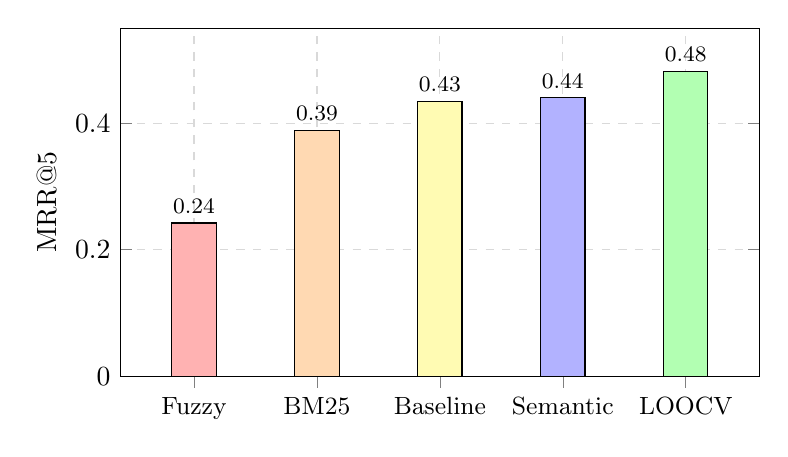
\begin{tikzpicture}
\begin{axis}[
    ybar,
    bar width=16pt,
    ymin=0, ymax=0.55,
    ylabel={MRR@5},
    xtick={1,2,3,4,5},
    xticklabels={Fuzzy,BM25,Baseline,Semantic,LOOCV},
    xticklabel style={font=\small},
    xtick pos=left,
    bar shift=0pt,
    width=0.8\textwidth,
    height=6cm,
    nodes near coords,
    nodes near coords style={font=\footnotesize, /pgf/number format/fixed, /pgf/number format/precision=2},
    grid=major,
    grid style={dashed, gray!30},
    xmin=0.4, xmax=5.6,
    enlarge x limits=false
]
\addplot[fill=red!30] coordinates {(1,0.242)};
\addplot[fill=orange!30] coordinates {(2,0.388)};
\addplot[fill=yellow!30] coordinates {(3,0.434)};
\addplot[fill=blue!30] coordinates {(4,0.440)};
\addplot[fill=green!30] coordinates {(5,0.482)};
\end{axis}
\end{tikzpicture}
\captionof{figure}{Performance comparison of MRR@5 across methods. LOOCV represents held-out performance, while others show resubstitution results.}
\label{fig:performance_comparison}
\end{minipage}
\vspace{0.5em}

\subsection{Ablation Study}

To understand signal contributions, we perform ablation by removing one signal at a time from the optimized weights and renormalizing:

\begin{table}[H]
\centering
\small
\begin{tabular}{lcrrr}
\toprule
\textbf{Configuration} & \textbf{Weights} & \textbf{MRR@5} & \textbf{$\Delta$ MRR} & \textbf{Interpretation} \\
\midrule
Full model & (0.80, 0.10, 0.10) & 0.527 & -- & Baseline \\
No Semantic & (0.00, 0.50, 0.50) & 0.394 & -0.133 & Critical signal \\
No BM25 & (0.89, 0.00, 0.11) & 0.445 & -0.082 & Important complement \\
No Fuzzy & (0.89, 0.11, 0.00) & 0.522 & -0.005 & Minimal impact \\
\bottomrule
\end{tabular}
\caption{Ablation study showing signal contributions. Performance measured on full dataset with median LOOCV weights.}
\label{tab:ablation}
\end{table}

\subsection{Weight Sensitivity}

We analyze robustness by perturbing each weight by $\Delta \in \{-0.2, -0.1, 0, +0.1, +0.2\}$ while maintaining the convex constraint:

\vspace{0.5em}
\noindent
\begin{minipage}{\textwidth}
\centering
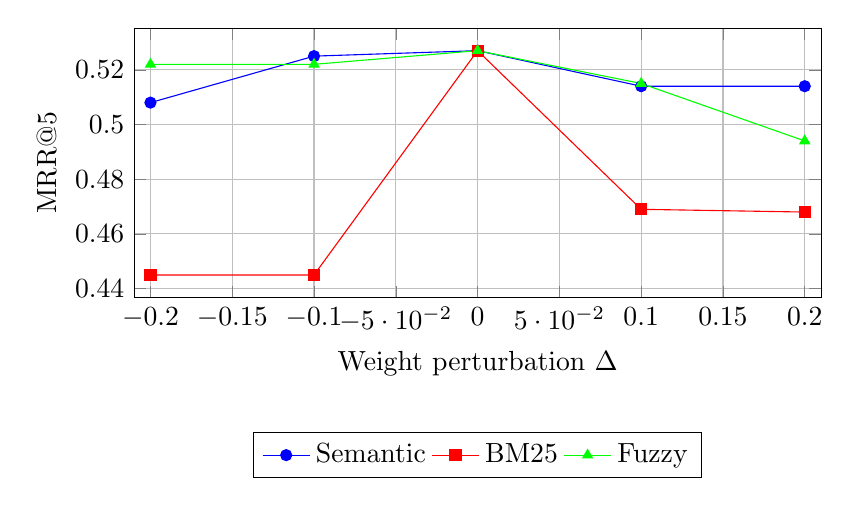
\begin{tikzpicture}
\begin{axis}[
    xlabel={Weight perturbation $\Delta$}, 
    ylabel={MRR@5},
    width=0.85\textwidth, 
    height=5cm, 
    grid=both,
    xmin=-0.21, xmax=0.21,
    legend style={at={(0.5,-0.5)}, anchor=north, legend columns=-1}
]
\addplot[color=blue,mark=*] coordinates {
    (-0.20,0.508) (-0.10,0.525) (0.00,0.527) (0.10,0.514) (0.20,0.514)
};
\addplot[color=red,mark=square*] coordinates {
    (-0.20,0.445) (-0.10,0.445) (0.00,0.527) (0.10,0.469) (0.20,0.468)
};
\addplot[color=green,mark=triangle*] coordinates {
    (-0.20,0.522) (-0.10,0.522) (0.00,0.527) (0.10,0.515) (0.20,0.494)
};
\legend{Semantic, BM25, Fuzzy}
\end{axis}
\end{tikzpicture}
\captionof{figure}{Sensitivity of MRR@5 to weight perturbations. The optimized configuration shows good stability within $\pm$0.1 range.}
\label{fig:sensitivity}
\end{minipage}
\vspace{0.5em}

\section{System Performance}
\label{sec:evaluation-performance}

Beyond retrieval quality, we validate system responsiveness on the full corpus of 1,157 rules:

\begin{table}[H]
\centering
\begin{tabular}{lrrl}
\toprule
\textbf{Metric} & \textbf{Measured} & \textbf{Target} & \textbf{Status} \\
\midrule
Startup time & 464ms & <1s & \checkmark \\
Median latency & 58ms & <100ms & \checkmark \\
P95 latency & 660ms & <1000ms & \checkmark \\
Memory usage & 530MB & <1GB & \checkmark \\
\bottomrule
\end{tabular}
\caption{System performance validation. All metrics meet production requirements.}
\label{tab:performance}
\end{table}

Detailed performance analysis is provided in Appendix~\ref{app:implementation}.

\section{Discussion}
\label{sec:evaluation-discussion}

\subsection{Key Findings}

Our evaluation reveals several important insights:

\begin{itemize}[leftmargin=*,itemsep=2pt,topsep=2pt]
  \item \textbf{Hybrid superiority}: The optimized hybrid (48.2\% MRR@5) outperforms the best individual signal (semantic at 44.0\%) by 4.2 percentage points
  \item \textbf{Semantic dominance}: The 80\% weight on semantic signals reflects the value of deep language understanding for rule discovery
  \item \textbf{Complementary signals}: BM25 contributes 8.2pp when added to semantic, while fuzzy adds only 0.5pp but helps with exact name matches
  \item \textbf{Robust configuration}: Performance remains stable with $\pm$10\% weight variations
\end{itemize}

\subsection{Limitations}

This evaluation has several limitations that should guide interpretation:

\begin{enumerate}[leftmargin=*,itemsep=2pt,topsep=2pt]
  \item \textbf{Small dataset}: 30 queries provide preliminary validation but prevent strong statistical claims
  \item \textbf{Binary relevance}: Our evaluation assumes single correct answers, though some rules may be partially relevant
  \item \textbf{Query distribution}: Test queries may not reflect actual usage patterns
  \item \textbf{Static corpus}: Evaluation doesn't capture performance as the rule base grows
\end{enumerate}

\subsection{Comparison to Related Systems}

While direct comparison is difficult due to different domains and datasets, our results align with trends in hybrid retrieval literature:

\begin{itemize}[leftmargin=*,itemsep=2pt,topsep=2pt]
  \item Dense retrieval (semantic) increasingly dominates but benefits from lexical signals
  \item Optimal weights typically range from 70-85\% semantic, 10-25\% BM25
  \item Fuzzy matching rarely exceeds 10\% weight in well-tuned systems
\end{itemize}

\section{Conclusions}
\label{sec:evaluation-conclusions}

This evaluation demonstrates that our hybrid retrieval system achieves reasonable performance on a preliminary test set, with LOOCV-tuned weights of (0.80, 0.10, 0.10) for semantic, BM25, and fuzzy signals respectively. The system meets performance requirements with sub-100ms median latency while improving retrieval quality over individual signals.

However, these results should be considered preliminary. Future work should:
\begin{itemize}[leftmargin=*,itemsep=2pt,topsep=2pt]
  \item Expand evaluation to 200+ queries for statistical validity
  \item Include graded relevance judgments for more nuanced evaluation
  \item Test on actual user queries from production logs
  \item Evaluate robustness as the corpus grows beyond 1,157 rules
\end{itemize}

Despite these limitations, the evaluation validates our architectural approach and provides a solid foundation for deployment and iterative improvement based on real user feedback.
